\begin{figure}[!htbp]
  \centering
  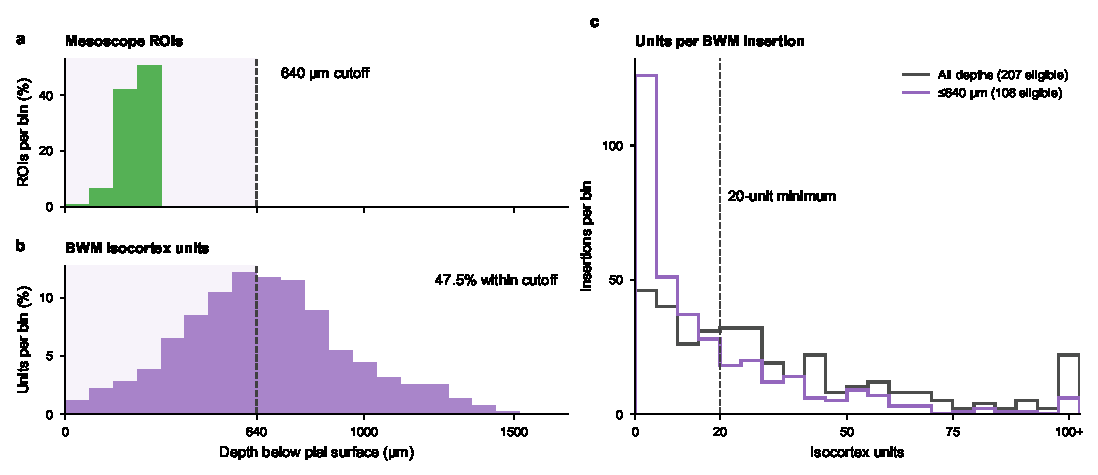
\includegraphics[width=\linewidth,height=0.8\textheight,keepaspectratio]{figures/depth_coverage.pdf}
  \caption{Recording depth and probe eligibility. The IBL 25-micron Allen CCF streamline lookup estimates local pial depth. \textbf{a} Depths of 202,329 isocortex ROIs pooled over 24 histology-registered mesoscope sessions. Sessions with projected positions are omitted. \textbf{b} Depths of 12,890 good BWM isocortex units. The shaded range ends at the dashed 640\,$\mu$m cutoff and contains 6,125 units (47.5\,\%). Both depth histograms use 80\,$\mu$m bins and are normalized separately. \textbf{c} Unit counts per insertion for 350 BWM insertions in sessions with at least 50 eligible trials. The dashed line marks the 20-unit requirement for the decoding maps. 207 insertions meet it at all depths and 108 meet it after the depth cutoff. Counts of at least 100 units share the final bin.}
  \label{fig:depth_coverage}
\end{figure}
